%% 
%% Copyright 2007-2024 Elsevier Ltd
%% 
%% This file is part of the 'Elsarticle Bundle'.
%% ---------------------------------------------
%% 
%% It may be distributed under the conditions of the LaTeX Project Public
%% License, either version 1.3 of this license or (at your option) any
%% later version.  The latest version of this license is in
%%    http://www.latex-project.org/lppl.txt
%% and version 1.3 or later is part of all distributions of LaTeX
%% version 1999/12/01 or later.
%% 
%% The list of all files belonging to the 'Elsarticle Bundle' is
 %% given in the file `manifest.txt'.
%% 
%% Template article for Elsevier's document class `elsarticle'
%% with harvard style bibliographic references

\documentclass[preprint,12pt,authoryear]{elsarticle}

%% Use the option review to obtain double line spacing
%% \documentclass[authoryear,preprint,review,12pt]{elsarticle}

%% Use the options 1p,twocolumn; 3p; 3p,twocolumn; 5p; or 5p,twocolumn
%% for a journal layout:
%% \documentclass[final,1p,times,authoryear]{elsarticle}
%% \documentclass[final,1p,times,twocolumn,authoryear]{elsarticle}
%% \documentclass[final,3p,times,authoryear]{elsarticle}
%% \documentclass[final,3p,times,twocolumn,authoryear]{elsarticle}
%% \documentclass[final,5p,times,authoryear]{elsarticle}
%% \documentclass[final,5p,times,twocolumn,authoryear]{elsarticle}

%% For including figures, graphicx.sty has been loaded in
%% elsarticle.cls. If you prefer to use the old commands
%% please give \usepackage{epsfig}

%% The amssymb package provides various useful mathematical symbols
\usepackage{amssymb}
%% The amsmath package provides various useful equation environments.
\usepackage{amsmath}
\usepackage{algorithm}
\usepackage{algorithmicx}
\usepackage{algpseudocode}
%% The amsthm package provides extended theorem environments
%% \usepackage{amsthm}

%% The lineno packages adds line numbers. Start line numbering with
%% \begin{linenumbers}, end it with \end{linenumbers}. Or switch it on
%% for the whole article with \linenumbers.
%% \usepackage{lineno}

\journal{Computers and Operation Research}

\begin{document}

\begin{frontmatter}

%% Title, authors and addresses

%% use the tnoteref command within \title for footnotes;
%% use the tnotetext command for theassociated footnote;
%% use the fnref command within \author or \affiliation for footnotes;
%% use the fntext command for theassociated footnote;
%% use the corref command within \author for corresponding author footnotes;
%% use the cortext command for theassociated footnote;
%% use the ead command for the email address,
%% and the form \ead[url] for the home page:
%% \title{Title\tnoteref{label1}}
%% \tnotetext[label1]{}
%% \author{Name\corref{cor1}\fnref{label2}}
%% \ead{email address}
%% \ead[url]{home page}
%% \fntext[label2]{}
%% \cortext[cor1]{}
%% \affiliation{organization={},
%%            addressline={}, 
%%            city={},
%%            postcode={}, 
%%            state={},
%%            country={}}
%% \fntext[label3]{}

\title{Actor-based Large Neighborhood Search} %% Article title

%% use optional labels to link authors explicitly to addresses:
%% \author[label1,label2]{}
%% \affiliation[label1]{organization={},
%%             addressline={},
%%             city={},
%%             postcode={},
%%             state={},
%%             country={}}
%%
%% \affiliation[label2]{organization={},
%%             addressline={},
%%             city={},
%%             postcode={},
%%             state={},
%%             country={}}

\author{Christian Brunbjerg Jespersen} %% Author name

%% Author affiliation
\affiliation{organization={},%Department and Organization
            addressline={}, 
            city={},
            postcode={}, 
            state={},
            country={}}

%% Abstract
\begin{abstract}
%% Text of abstract
Abstract text.
\end{abstract}

%%Graphical abstract
\begin{graphicalabstract}
%\includegraphics{grabs}
\end{graphicalabstract}

%%Research highlights
\begin{highlights}
\item How to allow direct and real-time integration into an optimization process?
\item How to perform optimmization in a real-time changing parameter space?
\end{highlights}

%% Keywords
\begin{keyword}
%% keywords here, in the form: keyword \sep keyword
Large Neighborhood Search \sep Actor Framework \sep Real-time Optimization \sep human-centered computing \sep Interactive Systems and Tools \sep Decision Support Systems \sep Interactive Optimization


%% PACS codes here, in the form: \PACS code \sep code

%% MSC codes here, in the form: \MSC code \sep code
%% or \MSC[2008] code \sep code (2000 is the default)

\end{keyword}

\end{frontmatter}

%% Add \usepackage{lineno} before \begin{document} and uncomment 
%% following line to enable line numbers
%% \linenumbers

%% main text
%%

%% Use \section commands to start a section
\section{Introduction}
\label{sec:1-introduction}
%% Labels are used to cross-reference an item using \ref command.

Many problems in operation research are hard to solve due to the need of tight integration with tacit knowledge found in the minds of key decision makers 
that have to make decisions based on solutions provided by operation research methods such as metaheuristics and commercial solvers. 
To solve operation research problems that are highly operational in nature there three additional requirements for metaheuristics to have: 1.  
responsive, 2. able to be assimilated into the decision makers workflow, and 3. allows for integration into dynamic data source such as traditional databases \citep{meignan_review_2015}. 
Operational aspects of operation research, as opposed to strategic and tactical aspects, are often characterized by by extensive amounts negotiation and feedback on 
proposed solutions to general operations research problems (!!!). This can lead to a situation
where operation research methods are not used to solve the problem of their underlying model and instead provides intial suggestions \cite{meignan_review_2015}. In practice
operations are usually characterized by extensive negotiation and feedback on proposed "solutions" between relevant stakeholders.  

This paper proposes a solution method that will allow for real-time optimization based on user-interaction (changes to the parameter space) and connection to a dynamic 
data source (in practice a database connection). The proposed solution method will be based on the multi-compartment multi-knapsack problem on a large dataset. 
Further the large neighborhood search metaheuristic has been chosen due to its properties of being able to work with and fix infeasible solutions. 

The paper is divided into four different sections. Section \ref{sec:2-solution-method} explains the model and method in detail that form the fundation of the paper. 
Section \ref{sec:3-results} shows that results coming from the implemented system where the system will be affected by simulated user-interaction. Section \ref{sec:4-discussion} 
will discuss the implications of the research and possible future research directions.

\subsection{The Multi-compartment Multi-knapsack Problem with capacity penalties}
\label{sub1sec2}
A variant of the knapsack problem is applied to the actor-based large neighborhood search. It was chosen due to its simplicity
while also being sufficiently computationally hard to be able to illustrate the power behind the solution approach. The model is comprised of 
five different sets. Here: $K$ is the number of knapsacks; $I$ is the number of items; $C$ is the number of compartments; $Q$ is a set that
defines which items should be excluded from a specific knapsack; $P$ is an inclusion set that defines the items which should be included in each 
knapsack. The model introduces four different parameters. Here: $v_{ik}$ is the value associated with item i in knapsack k; $d$ is the 
penalty paid for exceeding the compartment capacity; $w_{ic}$ is the capacity requirement for item i in compartment c; $cap_{kc}$ is the total amount 
of capacity available in knapsack k for compartment c. The decision-variables are: $x_{ik}$, which is a binary decision variable equal to one 
if item i is in knapsack k and zero otherwise; $p_{kc}$ is non-negative decision variable equal to the amount of excess capacity above 
the $c_{kc}$ in knapsack k for compartment c. 

\begin{alignat}{2}
	& \text{Min} \quad \sum_{i = 1}^{I} \sum_{k = 1}^{K} v_{ik} \cdot x_{ik} + \sum_{k = 1}^{K} \sum_{c = 1}^C d \cdot p_{kc}   \label{eqn:objective_function_strategic} \\[1em]
    & \text{subject to:} \notag                                                                                                                                        \\[1em]
	& \sum_{i=1}^I w_{ic} \cdot x_{ik} \leq \ cap_{kc} + p_{kc}        && \forall k \in K, \forall c \in C                      \label{eqn:capacity_constraint}          \\[1em]
	& \sum_{i = 1}^{I} x_{ik} = 1                                      && \forall k \in K                                       \label{eqn:single_workorder_constraint}  \\[1em]
	& x_{ik} = 0                                                       && \forall (i, k) \in Q                                  \label{eqn:exclusion_constraint}         \\[1em]
	& x_{ik} = 1                                                       && \forall (i, k) \in P                                  \label{eqn:inclusion_constraint}         \\[1em]
	& x_{ik} \in \{0, 1\}                                              && \forall i \in I, \forall k \in K                      \label{eqn:x_integrality_constraint}     \\[1em] 
	& p_{kc} \in \mathbb{R}^{+}                                        && \forall k \in K, \forall c \in C                      \label{eqn:p_non_negativity_constraint}
\end{alignat}

Here the objective function \ref{eqn:objective_function_strategic} aims to minimize the total weight of all item set assignments under a penalty $d$ given for exceeding the 
capacity given by constraint \ref{eqn:capacity_constraint}. Constraint \ref{eqn:capacity_constraint} makes sure that all the weights $w_{ic}$ for each item in an item set, given that it
has been assigned, is lower than the capacity for each knapsack k and for each compartment c. $p_{kc}$ is the amount of exceed capacity that is needed for the current assignment of item sets to be feasible.
Constraint \ref{eqn:single_workorder_constraint} makes sure that each item set is assigned to atleast a single knapsack. Constraint \ref{eqn:exclusion_constraint} excludes item sets from 
certain knapsacks and constraint \ref{eqn:inclusion_constraint}  forces a specific item set to be in a specific knapsack. Constraint \ref{eqn:x_integrality_constraint} and \ref{eqn:p_non_negativity_constraint} 
specify the variable domain for $x_{ik}$ and $p_{kc}$ respectively. In this paper the effects of changing Q, P, cap, and v in real-time will be examined to determine their effects on the solution and objective value.

\section{Solution Method}
\label{sec:2-solution-method}

\subsection{Actor-based Large Neighborhood Search}
A problem that is subject to user-interaction and requires real-time feedback you need an optimization approach that is able to repair infeasible solutions and while also 
converging quickly. For this the large neighborhood search metaheuristic has been shown satisfy these requirements in the literature \cite{gendreau_handbook_2019}. 

The LNS metaheuristic is in its most basic form is implicitly defined for static problems meaning that the parameters that make up the problem instance is not subject to change 
after the algorithm has been started. To make the LNS able adapt to incoming information in real-time a message system have been implemented on top of the existing framework. This 
extension is shown in algorithm \ref{algo1}. In the pseudocode the $x$ 

\begin{algorithm}[H]
\caption{Actor-based Large Neighborhood Search}  \label{algo1}
\begin{algorithmic}[1]
\State \textbf{Input} queue = message queue
\State \textbf{Input} P     = problem instance
\State \textbf{Input} x     = initial solution
\State $x^b = x$
\While{true}
	\While{queue.has\_message()}
        \State m = queue.pop()
        \State $x$.update(m)
        \State $x^b$.update(m)
		
		\State P.update(m)
    \EndWhile
	
    \State $x^t = r(d(x))$
    \If{accept($x^t$,\ $x$)}                       \label{alg:acceptance_criteria_start}
        \State x = x$^t$
    \EndIf                                       \label{alg:acceptance_criteria_end}
    \If{$c(x^t) < c(x^b)$}                   \label{alg:objective_start}
        \State $x^b = x^t$
		\State queue($x^b$)
    \EndIf                                       \label{alg:objective_end}
\EndWhile
\Return $x^b$
\end{algorithmic}
\end{algorithm}

The basic LNS setup have here been extended with a `message queue`. This message queue will be read from on every iteration of the LNSs main iteration loop. And here we should notice that the 
incoming message are able to change both the solutoin but also the problem instance itself. Here we see one of the defining features of the LNS metaheuristic in play, that due to its inherrent 
property of being able to optimize a solution that have become infeasible which is something that is very likely to happen when you change the parameter of the problem instance itself. 

Another less obvious property the message queue allows is for the algorithm to run indefinitely and instead of restarting the algorithm you instead pass messages to it to allow it be adjust both the solution space and the parameter space.
This property avoid the issue of time consuming initial convergence as the algorithm will be found in an optimimal state when the solution is perturbed.  

\section{Results}
\label{sec:3-results}
This results section will 1. introduce the data instance 2. show the effect of forcing item set in the specific knapsacks 3. show the effect of changing the 
knapsack capacities, and 4. show the effect of dynamically changing the item set weights. 

\section{Data Instance}
\begin{table}[t]
\centering
\begin{tabular}{|c|c|c|c|c|}
\hline
           & \begin{tabular}[c]{@{}c@{}}Number of\\ Item Sets\end{tabular} & \begin{tabular}[c]{@{}c@{}}Number of\\ Compartments\end{tabular} & \begin{tabular}[c]{@{}c@{}}Number of\\ Knapsacks\end{tabular} \\ \hline
Instance 1 & 3487                                                          & 16                                                               & 52                                                            \\ \hline
           &                                                               &                                                                  &                                                               \\ \hline
           &                                                               &                                                                  &                                                               \\ \hline
\end{tabular}

\caption{Table Caption} % \label{fig1}
\end{table}
% \begin{table}[t]%% placement specifier
% %% Use tabular environment to tag the tabular data.
% %% https://en.wikibooks.org/wiki/LaTeX/Tables#The_tabular_environment
% \centering%% For centre alignment of tabular.
% \begin{tabular}{l c r}%% Table column specifiers
% %% Tabular cells are separated by &
%   1 & 2 & 3 \\ %% A tabular row ends with \\
%   4 & 5 & 6 \\
%   7 & 8 & 9 \\
% \end{tabular}
% %% Use \caption command for table caption and label.
% \end{table}

\subsection{Response to Inclusion}
The response to the inclusion of a work order is given by P parameter of the model which 
is constrained in \ref{eqn:inclusion_constraint} of model given in \ref{sub1sec2}.

The inclusion is made of forcing certain allocations of item sets to be in specific knapsack. Below a table is provided 
to show what changes will occur and at what and at what point in time.
\begin{table}[H]
\centering
\begin{tabular}{|c|c|c|c|c|c|}
\hline
\begin{tabular}[c]{@{}c@{}}\end{tabular}     & \begin{tabular}[c]{@{}c@{}}At Time:\\ 01:00\end{tabular} & \begin{tabular}[c]{@{}c@{}}At Time:\\ 02:00\end{tabular} & \begin{tabular}[c]{@{}c@{}}At Time:\\ 03:00\end{tabular} & \begin{tabular}[c]{@{}c@{}}At Time:\\ 04:00\end{tabular} & \begin{tabular}[c]{@{}c@{}}At Time:\\ 05:00\end{tabular} \\ \hline
\begin{tabular}[c]{@{}c@{}}$\Delta |P|$\end{tabular} & 10                                                       & 20                                                       & 30                                                       & 40                                                       & 50                                                       \\ \hline
\end{tabular}
\end{table}

With the inputs defined we will explain the main results which are shown in the figure below. 
% Use figure environment to create figures
% Refer following link for more details.
% https://en.wikibooks.org/wiki/LaTeX/Floats,_Figures_and_Captions
\begin{figure}[H]%% placement specifier
%% Use \includegraphics command to insert graphic files. Place graphics files in 
%% working directory.
\centering%% For centre alignment of image.
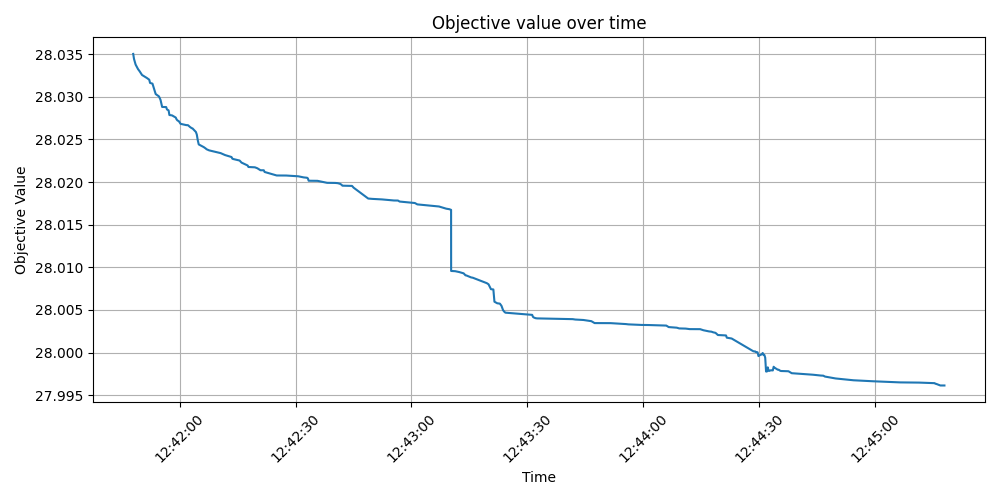
\includegraphics[width=1.0\textwidth]{../figures/objective.png}
%% Use \caption command for figure caption and label.
\caption{Figure Caption}\label{fig1}
%% https://en.wikibooks.org/wiki/LaTeX/Importing_Graphics#Importing_external_graphics
\end{figure}


\subsection{Response to Exclusion}
\begin{figure}[H]%% placement specifier
%% Use \includegraphics command to insert graphic files. Place graphics files in 
%% working directory.
\centering%% For centre alignment of image.
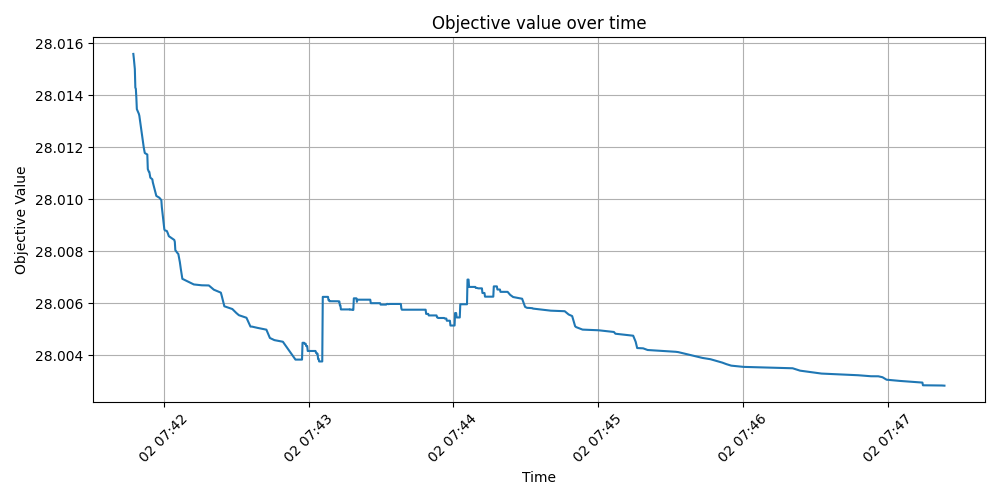
\includegraphics[width=1.0\textwidth]{../figures/objective-400-exclusions.png}
%% Use \caption command for figure caption and label.
\caption{Figure Caption}\label{fig:objective-exclusion-400}
%% https://en.wikibooks.org/wiki/LaTeX/Importing_Graphics#Importing_external_graphics
\end{figure}


\subsection{Response to Changes in Knapsack Capacities}
The effects of changes to capacities will be illustrated in the same way as it was with the response to inclusion and below we see the table that shows which inputs that the ALNS will be affected by.

\begin{table}[H]
\centering
\begin{tabular}{|c|c|c|c|c|c|}
\hline
                      & \begin{tabular}[c]{@{}c@{}}At Time:\\ 01:00\end{tabular} & \begin{tabular}[c]{@{}c@{}}At Time:\\ 02:00\end{tabular} & \begin{tabular}[c]{@{}c@{}}At Time:\\ 03:00\end{tabular} & \begin{tabular}[c]{@{}c@{}}At Time:\\ 04:00\end{tabular} & \begin{tabular}[c]{@{}c@{}}At Time:\\ 05:00\end{tabular} \\ \hline
$\Delta |k|$ & 16                                                       & 16                                                       & 16                                                       & 16                                                       & 16                                                       \\ \hline
$\Delta |c|$ & 16                                                       & 16                                                       & 16                                                       & 16                                                       & 16                                                       \\ \hline
$\Delta |cap|$& 100                                                      & 200                                                      & 400                                                      & 800                                                      & 1600                                                     \\ \hline
\end{tabular}
\end{table}

\begin{figure}[H]%% placement specifier
%% Use \includegraphics command to insert graphic files. Place graphics files in 
%% working directory.
\centering%% For centre alignment of image.
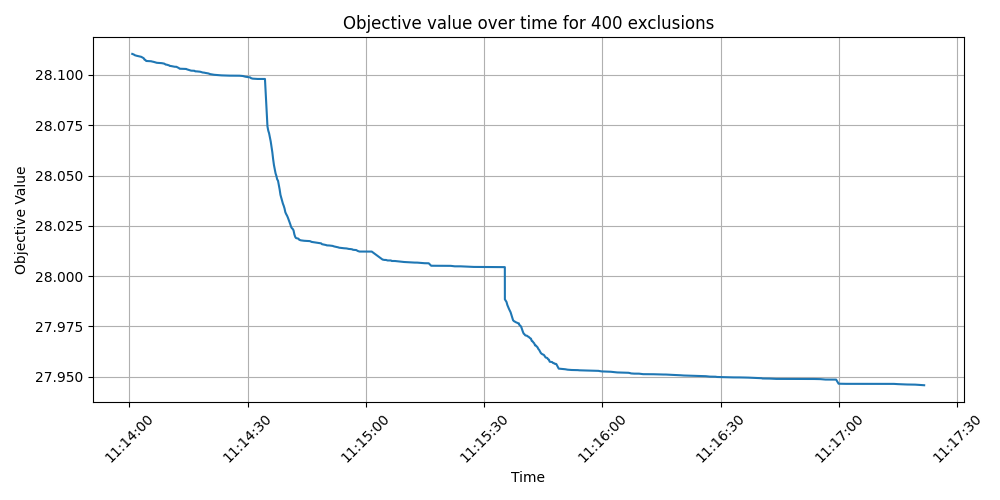
\includegraphics[width=1.0\textwidth]{../figures/objective-resource-increases.png}
%% Use \caption command for figure caption and label.
\caption{Figure Caption}\label{fig:objective-resource-increases}
%% https://en.wikibooks.org/wiki/LaTeX/Importing_Graphics#Importing_external_graphics
\end{figure}

Correspondingly we also have the figure below in which the resources are decreasing.

\subsection{Response to Changes in Item Weights}
The last parameter that will be changed in the item set wights. This section will be more elaborate as we have to show how that the item sets are rearranged due to the changes in their weights across the different periods.

\begin{table}[H]
\centering
\begin{tabular}{|c|c|c|c|c|c|}
\hline
             & \begin{tabular}[c]{@{}c@{}}At Time:\\ 01:00\end{tabular} & \begin{tabular}[c]{@{}c@{}}At Time:\\ 02:00\end{tabular} & \begin{tabular}[c]{@{}c@{}}At Time:\\ 03:00\end{tabular} & \begin{tabular}[c]{@{}c@{}}At Time:\\ 04:00\end{tabular} & \begin{tabular}[c]{@{}c@{}}At Time:\\ 05:00\end{tabular} \\ \hline
$\Delta |i|$ & 20                                                       & 40                                                       & 80                                                       & 160                                                      & 320                                                      \\ \hline
$\Delta |k|$ & 26                                                       & 26                                                       & 26                                                       & 26                                                       & 26                                                       \\ \hline
$\Delta |v|$ & $1 \cdot 10^{5}$                                         & $2 \cdot 10^{5}$                                         & $4 \cdot 10^{5}$                                         & $8 \cdot 10^{5}$                                         & $1.6 \cdot 10^{6}$                                       \\ \hline
\end{tabular}
\end{table}

\section{Discussion}
\label{sec:4-discussion}
There are multiple implications and new oppurtunities by adopting an approach to optimization as proposes by this paper. Some of these may not initially be completely obvious. In the discussion section we will go through the three 
most conseqential ones: 1. continual optimization saves the initial time it takes to reach converence significantly, 2. due to the message system the optimization approach will always be responsive to changes in both the parameter space
and the solution space, and 3. due to the strong encapsulation and message passing properties of the suggested optimization approach it becomes possible to apply the setup in multi-model and hierarchical model setups, providing an
approach for modelling and optimizing large scale systems. Finally a suggestion for future resarch directions will be given.

\subsection{Continuous Optimization}


\subsection{Message Passing versus Restarts}
\begin{itemize}
	\item Dynamic
	\item Resource efficient
	\item Integration (microservice)  
\end{itemize}

\subsection{System Level Optimization}






%% Use \subsubsection, \paragraph, \subparagraph commands to 
%% start 3rd, 4th and 5th level sections.
%% Refer following link for more details.
%% https://en.wikibooks.org/wiki/LaTeX/Document_Structure#Sectioning_commands


%% Displayed equations can be tagged using various environments. 

%% Single line equations can be tagged using the equation environment.
%% Unnumbered equations are tagged using starred versions of the environment.
%% amsmath package needs to be loaded for the starred version of equation environment.
%% align or eqnarray environments can be used for multi line equations.
%% & is used to mark alignment points in equations.
%% \\ is used to end a row in a multiline equation.
%% Unnumbered versions of align and eqnarray

%% Refer following link for more details.
%% https://en.wikibooks.org/wiki/LaTeX/Mathematics
%% https://en.wikibooks.org/wiki/LaTeX/Advanced_Mathematics

%% Use a table environment to create tables.
%% Refer following link for more details.
%% https://en.wikibooks.org/wiki/LaTeX/Tables
% \begin{table}[t]%% placement specifier
% %% Use tabular environment to tag the tabular data.
% %% https://en.wikibooks.org/wiki/LaTeX/Tables#The_tabular_environment
% \centering%% For centre alignment of tabular.
% \begin{tabular}{l c r}%% Table column specifiers
% %% Tabular cells are separated by &
%   1 & 2 & 3 \\ %% A tabular row ends with \\
%   4 & 5 & 6 \\
%   7 & 8 & 9 \\
% \end{tabular}
% %% Use \caption command for table caption and label.
% \caption{Table Caption}\label{fig1}
% \end{table}


%% Use figure environment to create figures
%% Refer following link for more details.
%% https://en.wikibooks.org/wiki/LaTeX/Floats,_Figures_and_Captions
% \begin{figure}[t]%% placement specifier
% %% Use \includegraphics command to insert graphic files. Place graphics files in 
% %% working directory.
% \centering%% For centre alignment of image.
% \includegraphics{example-image-a}
% %% Use \caption command for figure caption and label.
% \caption{Figure Caption}\label{fig1}
% %% https://en.wikibooks.org/wiki/LaTeX/Importing_Graphics#Importing_external_graphics
% \end{figure}


%% The Appendices part is started with the command \appendix;
%% appendix sections are then done as normal sections
% \appendix
% \section{Example Appendix Section}
% \label{app1}

% Appendix text.

%% For citations use: 
%%       \citet{<label>} ==> Lamport (1994)
%%       \citep{<label>} ==> (Lamport, 1994)
%%
% Example citation, See \cite{interactive-optimization-methods} 
%% If you have bib database file and want bibtex to generate the
%% bibitems, please use
%%
%%  \bibliographystyle{elsarticle-harv} 
%%  \bibliography{<your bibdatabase>}

%% else use the following coding to input the bibitems directly in the
%% TeX file.

%% Refer following link for more details about bibliography and citations.
%% https://en.wikibooks.org/wiki/LaTeX/Bibliography_Management
\bibliography{/home/scipo/coding/papers/actor-based-large-neighborhood-search/bib/refs}

\bibliographystyle{elsarticle-harv}
\end{document}

\endinput
%%
%% End of file `elsarticle-template-harv.tex'.


